\documentclass[11pt]{article}

% Packages
\usepackage{amsmath,amssymb,amsthm} % Math stuff
\usepackage{enumitem} % For improved lists
\usepackage{fancyhdr} % For headers
\usepackage{geometry} % Page geometry
\usepackage{graphicx}
\usepackage{booktabs}
\usepackage{subcaption}
\geometry{margin=1in}
\usepackage{xcolor}
\usepackage{float}
\usepackage{mathtools}
\usepackage[colorlinks=true, 
    linkcolor=blue, 
    citecolor=blue, 
    urlcolor=blue, 
    filecolor=blue]{hyperref}

% Header
\pagestyle{fancy}
\fancyhf{}
\lhead{Asher Baraban, Matej Cerman \\ Martin Hiti}
\chead{14.382}
\rhead{Problem Set 3}
\cfoot{\thepage}

\newtheorem{theorem}{Theorem}[section]

% For easier problem/solution environments
\newenvironment{problem}[1]
    {\bigskip\noindent\textbf{Problem #1.}\par\setlength{\parindent}{0pt}}
    {\medskip}
\newenvironment{solution}[1]
    {\bigskip\noindent\textbf{Solution #1.} \par}
    {\medskip}

\newcommand\barbelow[1]{\stackunder[1.2pt]{$#1$}{\rule{.8ex}{.075ex}}}

% Citations
\usepackage{natbib}
\bibliographystyle{unsrtnat}

% Math shortcuts
\newcommand{\ev}{\mathbb{E}}
\newcommand{\evn}{\mathbb{E}_n}
\newcommand{\R}{\mathbb{R}}

% Title
\title{Problem Set 3 \\ 14.382}
\author{Asher Baraban, Matej Cerman, Martin Hiti}
\date{\today}

% Document
\begin{document}


\maketitle

\noindent \textit{Notes}:
\begin{itemize}
    \item All code is in \url{https://github.com/ABaraban/14.382_pset3}
    \item All three group members took 14.381 last semester
\end{itemize}

\subsection*{Chapter 7} 

%%%%%%%%%%%%%%%%%%%%%%%%%%%%%%%%%%%%%%%%%%%%%%%%%%%%%%%%%
\begin{problem}{7.1}
State the score function g(·, ·) and moment Jacobian matrix
G for the probit and logit quasi-maximum likelihood estimators.
\end{problem}

\begin{solution}{7.1}
A generic M-estimator takes the form 
\[\hat{\beta} \in \arg\min_{\beta}E_nm(Z,\beta)\]
\end{solution} 
To do, maximum likelihood estimation, $m(Z,\beta) = -lnf(Z,\beta)$
In the case of probit or logit estimators, we can think of $Z$ as $(Y,X)$. In this case, we can write. Note $g(X)$ is the density of $X$.
\[lnf(Z,\beta) = lnf(Y|X, \beta) + lng(X)\]
Therefore, we can write the optimization problem as $g(X)$ doesn't depend on $\beta$. 
\[\hat{\beta} \in \arg\min_{\beta}-E_n\left[lnf(Y|X,\beta)\right]\]
Now we can couch this optimization as a GMM using its FOC! For an interior optimum we have 
\[-\frac{\partial}{\partial \beta}E_n\left[lnf(Y|X,\beta)\right] = 0\]
This is precisely a GMM moment condition so we can define our $g$.
\[g((X,Y), \beta) =-\frac{\partial }{\partial \beta}lnf((X,Y), \beta)\]
So our GMM sample moment condition is 
\[E_ng((X,Y), \beta) =E_n-\frac{\partial }{\partial \beta}lnf((X,Y), \beta) = 0\]
For both probit and logit, $Y \in {0,1}$ with a link function $F$ where our $f$ above is $f=F'$. We are trying to model $P(Y=1|X,\beta) = F(B(X)'\beta)$, and $P(Y=0|X,\beta) =1- F(B(X)'\beta)$ where $B$ is a dictionary of transformations. We can combine both cases into a single formula.
\[f(Y|X,\beta) = F(B(X)'\beta)^Y(1-F(B(X)'\beta)^{1-Y}\]
Now, we can find the log likelihood
\[lnf(Y|X,\beta) = YlnF(B(X)'\beta) + (1-Y)ln\left[1-F(B(X)'\beta)\right]\]
\subsection*{Probit}
Probit just parametrizes the CDF
\[F = \Phi(t) = \int_{-\infty}^t\frac{1}{\sqrt{2\pi}}e^{\frac{-s^2}{2}}ds\]
\[lnf(Y|X,\beta) = Yln\Phi(B(X)'\beta) + (1-Y)ln\left[1-\Phi(B(X)'\beta)\right]\]
To find $g$ we differentiate let $\phi$ be the normal PDF
\[\frac{\partial}{\partial \beta}lnf(Y|X,\beta) = Y \frac{\phi(B(X)'\beta)B(X)}{\Phi(B(X)'\beta)} + (1-Y)\frac{-\phi(B(X)'\beta)B(X)}{1-\Phi(B(X)'\beta)}\]
\[\frac{\partial}{\partial \beta}lnf(Y|X,\beta) = \phi(B(X)'\beta)B(X)\left[ \frac{Y}{\Phi(B(X)'\beta)} + \frac{Y-1}{1-\Phi(B(X)'\beta)}\right]\]
Finding a common denominator and simplifying we get 
\[\frac{\partial}{\partial \beta}lnf(Y|X,\beta) = \phi(B(X)'\beta)B(X)\left[ \frac{Y-\Phi(B(X)'\beta)}{\Phi(B(X)'\beta)(1-\Phi(B(X)'\beta)} \right]\]
Plugging in we get 
\[g((X,Y), \beta) = -\phi(B(X)'\beta)B(X)\left[ \frac{Y-\Phi(B(X)'\beta)}{\Phi(B(X)'\beta)(1-\Phi(B(X)'\beta)} \right]\]
We now need to differentiate again w.r.t $\beta$ but using an expectation trick critically the expectation is over $Y$.
\[G = E\left[\frac{\partial}{\partial \beta}g((X,Y),\beta) \right]= E\left[\frac{\partial}{\partial \beta}\frac{-\phi(B(X)'\beta)B(X)}{\Phi(B(X)'\beta)(1-\Phi(B(X)'\beta)}\left[Y-\Phi(B(X)'\beta) \right]\right]\]

\[G =E\left[\frac{\partial}{\partial \beta}\frac{-\phi(B(X)'\beta)B(X)}{\Phi(B(X)'\beta)(1-\Phi(B(X)'\beta)}\left[Y-\Phi(B(X)'\beta) \right]\right]\]
First, simplify by defining $S(k) = \frac{\phi(k)}{\Phi(k)(1-\Phi(k))}$, where $k = B(X)'\beta$
\[G =-E\left[\frac{\partial}{\partial \beta}  S(k)B(X)\left[Y-\Phi(k) \right]\right]\]
Using product rule we get
\[G =-E\left[  S'(k)\frac{\partial k}{\partial \beta}B(X)\left[Y-\Phi(k) \right] - S(k)B(X)\phi(k)B(X)'\right]\]
Now use the law of iterated expectations 
\[G =-E\left[E\left[  S'(k)\frac{\partial k}{\partial \beta}B(X)[Y-\Phi(k) ]|X\right] - E\left[S(k)B(X)\phi(k)B(X)'|X\right]\right]\]
Rearranging we get
\[G =-E\left[S'(k)\frac{\partial k}{\partial \beta}B(X)E\left[Y-\Phi(k) |X\right] - E\left[S(k)B(X)\phi(k)B(X)'|X\right]\right]\]
Now, by construction $\Phi(k) = E[Y|X]$.
\[G =E\left[S(k)B(X)\phi(k)B(X)'\right]\]
Subbing back in 
\[G =E\left[\frac{\phi(B(X)'\beta)}{\Phi(B(X)'\beta)(1-\Phi(B(X)'\beta))}B(X)\phi(B(X)'\beta)B(X)'\right]\]
\subsection*{Logit}
Logit is another parametrization of CDF
\[F = \Lambda(t) = \frac{e^t}{1+e^t}\]
\[lnf(Y|X,\beta) = Yln \Lambda(B(X)'\beta) + (1-Y)ln[1-\Lambda(B(X)'\beta)]\]
To find $g$ we differentiate
\[\frac{\partial }{\partial \beta} ln f(Y|X,\beta) = \frac{Y \Lambda'(B(X)'\beta) B(X)}{\Lambda(B(X)'\beta)} - \frac{(1-Y)\Lambda'(B(X)'\beta)B(X)}{1-\Lambda(B(X)'\beta)}\]
Simplifying
\[\frac{\partial }{\partial \beta} ln f(Y|X,\beta) = \Lambda'(B(X)'\beta)B(X)\left[\frac{Y}{\Lambda(B(X)'\beta)} + \frac{(Y-1)}{1-\Lambda(B(X)'\beta)}\right]\]
Simplifying with a common denominator
\[\frac{\partial }{\partial \beta} ln f(Y|X,\beta) = \Lambda'(B(X)'\beta)B(X)\left[\frac{Y - \Lambda(B(X)'\beta)}{\Lambda(B(X)'\beta) (1-\Lambda(B(X)'\beta))}\right]\]
Plugging in we get our $g$
\[g((X,Y),\beta) = -\Lambda'(B(X)'\beta)B(X)\left[\frac{Y - \Lambda(B(X)'\beta)}{\Lambda(B(X)'\beta) (1-\Lambda(B(X)'\beta))}\right]\]
To simplify, explicitly find $\Lambda'(t)$
\[\Lambda'(t) = \frac{e^t}{(1+e^t)^2} = \Lambda(t)(1-\Lambda(t))\]
Plugging in 
\[g((X,Y),\beta) = -B(X)\left[Y - \Lambda(B(X)'\beta)\right]\]
In order to get the jacobian we need to differentiate $g$ w.r.t $\beta$
\[\frac{\partial}{\partial \beta}g((X,Y), \beta) = B(X)\Lambda'(B(X)'\beta)B(X)'\]
So, 
\[G= E\left[B(X)\Lambda\left(B(X)'\beta\right)\left(1-\Lambda\left(B(X)'\beta\right)\right)B(X)'\right]\]

%%%%%%%%%%%%%%%%%%%%%%%%%%%%%%%%%%%%%%%%%%%%%%%%%%%%%%%%%




%%%%%%%%%%%%%%%%%%%%%%%%%%%%%%%%%%%%%%%%%%%%%%%%%%%%%%%%%
\newpage
\begin{problem}{7.2 (Martin)} 
Argue that large sample properties of the estimator of the average predictive effect (b) could be obtained via the GMM approach. Argue that you can apply bootstrap to approximate the distribution of this estimator. A challenge problem for an extra credit: provide a similar argument for the sorted predictive effect.
\end{problem}


\begin{solution}{7.2}

\paragraph{Definitions}
Suppose we have an outcome variable of interest $Y$ and a vector of covariates $X=(D,W')'$ where $D$ is a binary treatment indicator and $W$ is a set of controls. Let $(d,w) \mapsto p(d,w)$ be some predictive function of $Y$, given $D$ and $W.$ For example,
\begin{align*}
    p(d,w) = \ev[Y | D = d, W = w].
\end{align*}
The predictive effect (PE) of changing $D=0$ to $D=1$ given covariates $W = w$ is 
\begin{align*}
    \theta_w = p(1,w) - p(0,w)
\end{align*}
The average predictive effect (APE) is defined as 
\begin{align*}
    \theta = \int \theta_w dM(w) = \ev[\theta_{\tilde W}] \qquad \tilde{W} \sim M
\end{align*}
where $M$ is some distribution of covariates. 

\paragraph{Estimating APE} The model above van be estimated by nonlinear least squares 
\begin{align*}
    \hat{\beta} \in \arg \min_{\beta \in \mathcal{B}} \ev_n m(Z,\beta), \qquad Z \coloneq (Y,X')', X\coloneq(D,W')'.
\end{align*}
where $m$ is the square loss function $m(Z,\beta) = (Y-p(X,\beta))^2$ and $\mathcal{B} \subseteq \R^{\text{dim} \beta}$ is the parameter space. After obtaining estimators $\hat{\beta}$ for the technical parameters, we can use the plug-in principle to obtain estimates of estimands of interest. For example, the estimator for the predictive effect (PE) of changing $D=0$ to $D=1$ given $W = w$ is
\begin{align*}
    \hat{\theta}_1 = \hat{p}(1,w) - \hat{p}(0,w) = p(1,w,\hat{\beta}) - p(0,w,\hat{\beta})
\end{align*}
A more complicated quantity is the APE. For example, consider the case where the distribution $M$ over which we integrate is the overall population, so that $M = F_W.$ The natural estimator is 
\begin{align*}
    \hat{\theta} = \int \hat{\theta}d\hat{F}_W(w) = \frac{1}{n}\sum_{i=1}^n\hat{\theta}_{W_i}
\end{align*}
where $\hat{F}_W$ is the empirical distribution function of the $W_i$'s, an estimator of $F_W$. The estimator $\hat{\theta}$ has two sources of uncertainty: one is created by the estimation of $\hat{\theta}_w,$ and one is created by the estimation of $F_W.$ This makes it difficult to find the approximate distribution of the estimator for the APE. However, we can overcome these problems by recasting the problem into GMM estimation.

We first set up GMM for the case of $M = F_W.$ We can will stack moment conditions for (1) the technical parameters $\beta$ and (2) the APE. The true value of the parameter $\beta$ solves
\begin{align*}
    \arg\min_{\beta \in \mathcal{B}} \ev[m(Z,\beta)]
\end{align*}
the first order condition of this problem is that 
\begin{align*}
    \ev\left[ \frac{\partial}{\partial \beta}m(Z,\beta)\right] = 0
\end{align*}
which provides one moment condition for each technical parameter in the vector $\beta.$ Next, we can get a moment condition from the APE. With $M = F_W$ (the population distribution of $W$) the APE is 
\begin{align*}
    &\theta = \ev[p(1,W,\beta) - p(0,w,\beta)] \\
    \implies& \ev[\theta - (p(1,W,\beta) - p(0,w,\beta))] = 0
\end{align*}
This gives us a moment condition for $\theta.$ Stacking our moment conditions, we can view this as a GMM problem with the score function 
\begin{align*}
    \tilde{g}(Z,\gamma) &=
    \begin{pmatrix}
        \theta - (p(1,W,\beta) - p(0,w,\beta)) \\
        \frac{\partial}{\partial \beta}m(Z,\beta)
    \end{pmatrix}
\end{align*}
where $\gamma = (\theta,\beta')'.$ Then, we can invoke  condition $G$ and the GMM machinery to analyze the theoretical properties of this estimator--in particular, $\hat{\gamma} = (\hat{\theta},\hat{\beta}')'$ will be consistent and asymptotically normal, and we can write down the large sample variance. Moreover, we can use the bootstrap for calculating the large sample variance and distribution. To do so, we can proceed as follows
\begin{enumerate}
    \item 
\end{enumerate}


\end{solution}
%%%%%%%%%%%%%%%%%%%%%%%%%%%%%%%%%%%%%%%%%%%%%%%%%%%%%%%%%
\newpage
\begin{problem}{7.3}
Estimate average predictive effects and sorted predictive
effects (at various percentile indices) of race on the probability
of mortgage denial using the mortgage data. Explain
the choice of the link function you have made and provide
results for two different link functions. Report confidence
intervals based on the bootstrap. You can present the results
in a table or as in the figures above. How should we interpret
the results causally?
\end{problem}

\begin{solution}{7.3 (Asher)}

\begin{figure}[h!]
    \centering
    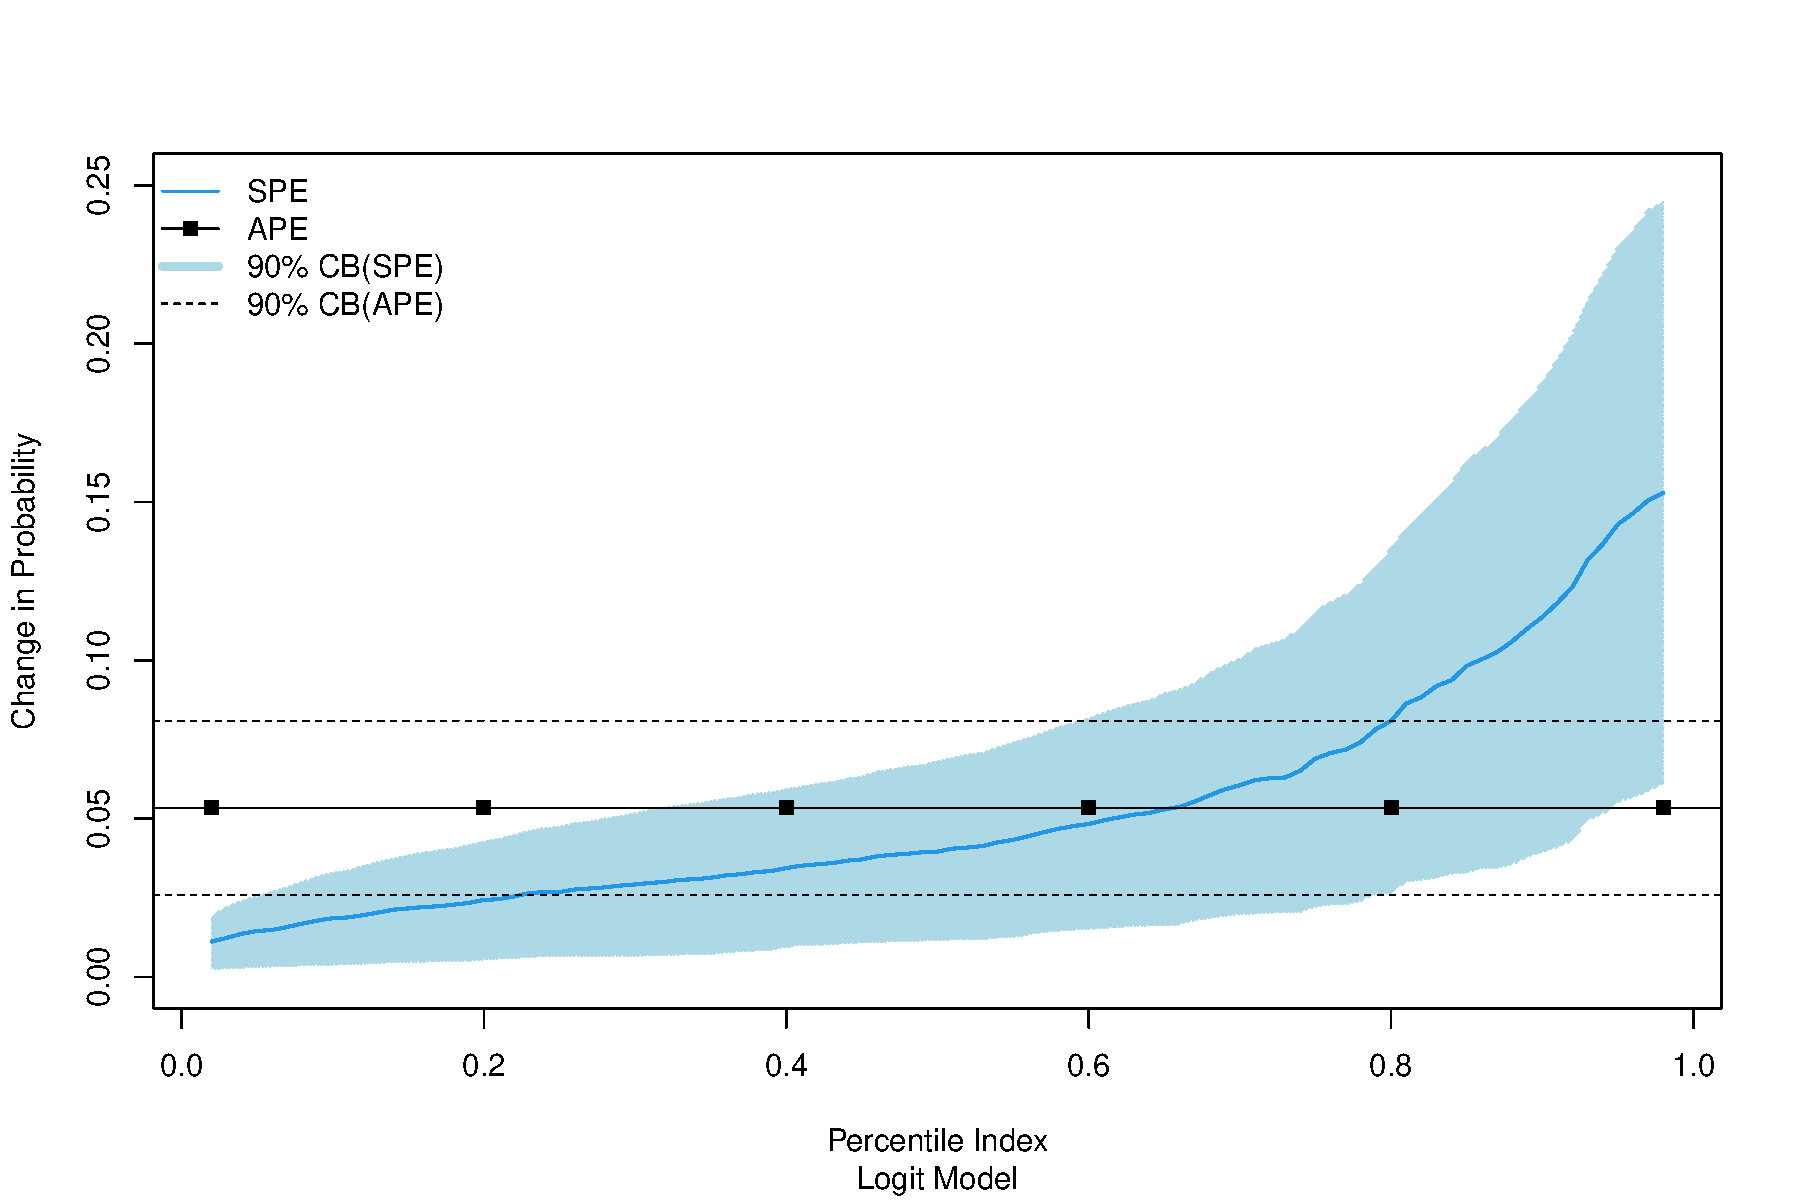
\includegraphics[width=0.5\linewidth]{Mortgage-SPE.pdf}
    \caption{Logit Model SPE}
    \label{fig:placeholder}
\end{figure}
\begin{figure}[h!]
        \centering
        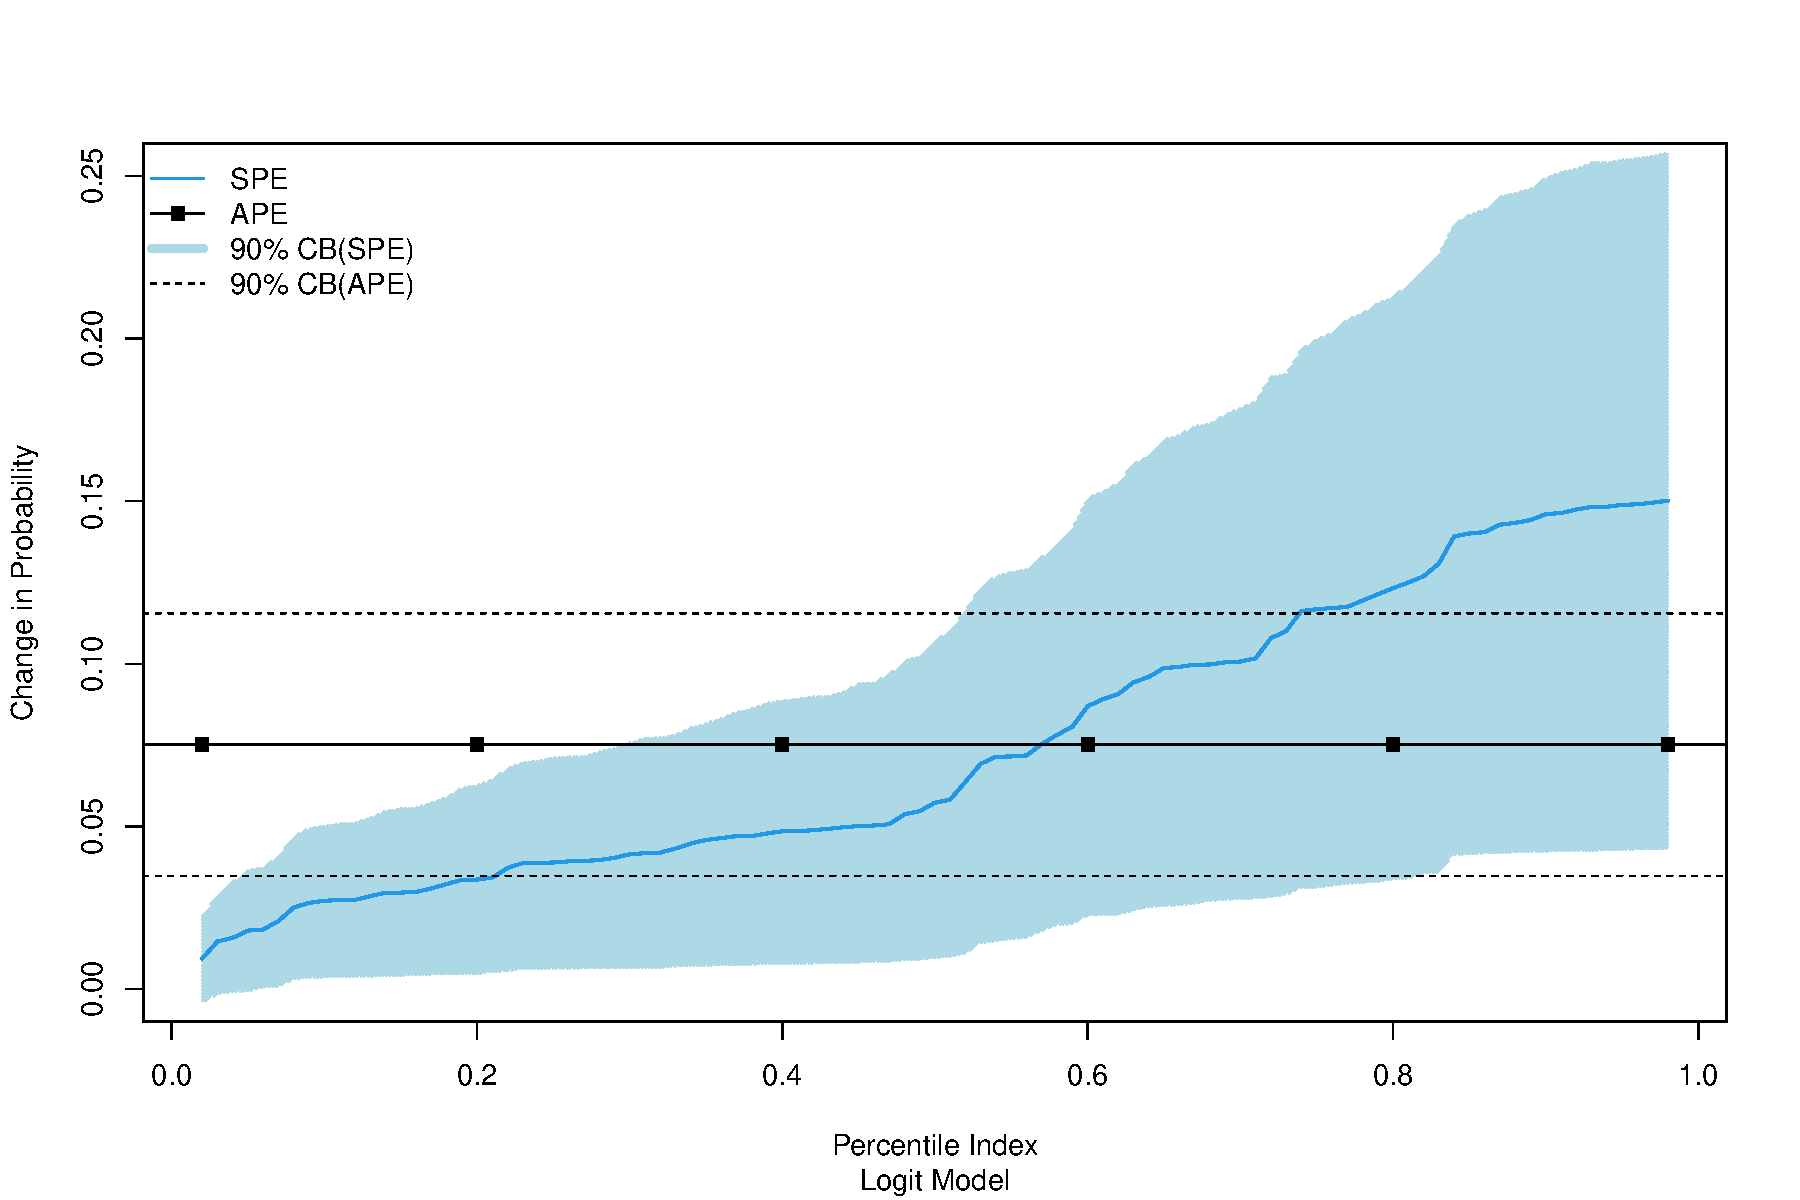
\includegraphics[width=0.5\linewidth]{Mortgage-SPET.pdf}
        \caption{Enter Caption}
        \label{fig:placeholder}
\end{figure}
\begin{figure}
    \centering
    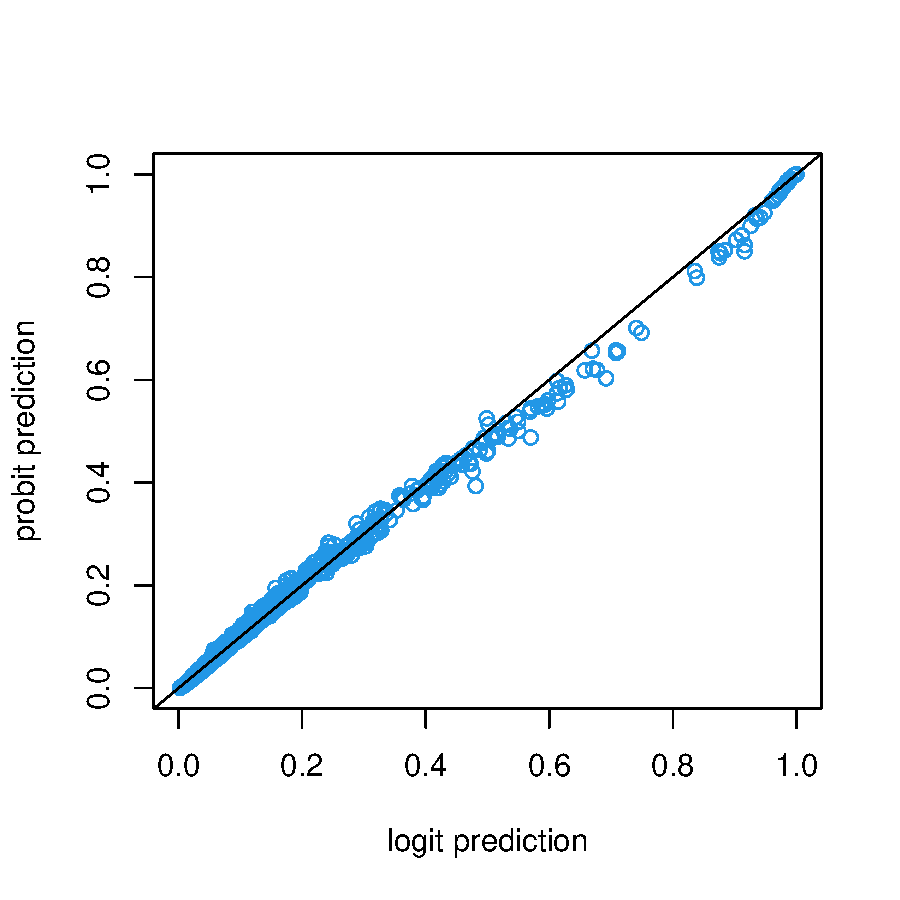
\includegraphics[width=0.5\linewidth]{LogitvsProbit1_mort.pdf}
    \caption{Comparing Probit vs Logit Model Prediction}
    \label{fig:placeholder}
\end{figure}

\begin{figure}
    \centering
    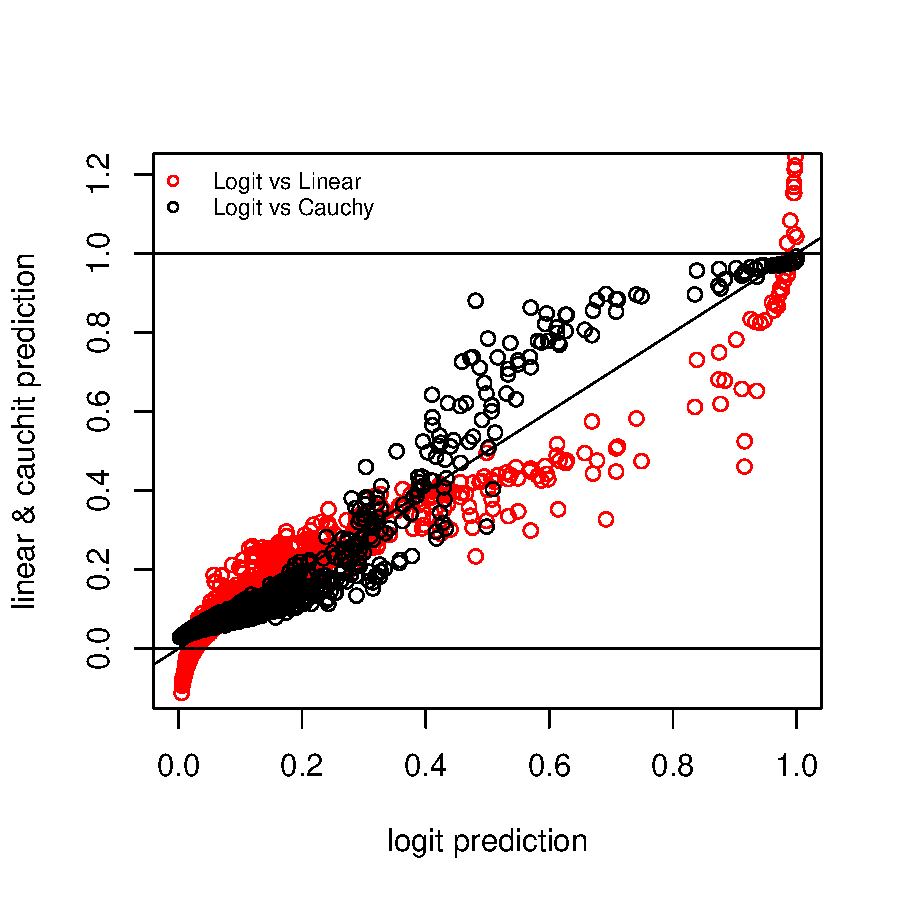
\includegraphics[width=0.5\linewidth]{LogitvsLinear1_mort.pdf}
    \caption{Cauchy
and Linear Against the Logit Model}
    \label{fig:placeholder}
\end{figure}
\end{solution}

%%%%%%%%%%%%%%%%%%%%%%%%%%%%%%%%%%%%%%%%%%%%%%%%%%%%%%%%%
\
%%%%%%%%%%%%%%%%%%%%%%%%%%%%%%%%%%%%%%%%%%%%%%%%%%%%%%%%%

\newpage
\subsection*{Chapter 8}


%%%%%%%%%%%%%%%%%%%%%%%%%%%%%%%%%%%%%%%%%%%%%%%%%%%%%%%%%
\begin{problem}{8.2}
Replicate the results of one the empirical examples. Provide
a brief explanation for what you are doing. You can use the R
code provided, but you need to write comments in the code
explaining what each block of the code is doing.
\end{problem}

\begin{solution}{8.2 (Matej)}

We decided to reproduce the Gender Gap example. First, we show some summary statistics for the main variable of interest (log wage) together with covariates that will be used in the analysis.

% latex table generated in R 4.5.1 by xtable 1.8-8 package
% Thu Mar 12 16:33:35 2026
\begin{table}[ht]
\centering
\begin{tabular}{rrrr}
  \hline
 & Total & Women & Men \\ 
  \hline
lnw & 3.15 & 3.02 & 3.25 \\ 
  female & 0.44 & 1.00 & 0.00 \\ 
  married & 0.65 & 0.61 & 0.68 \\ 
  widowed & 0.01 & 0.02 & 0.01 \\ 
  separated & 0.02 & 0.02 & 0.02 \\ 
  divorced & 0.13 & 0.16 & 0.10 \\ 
  nevermarried & 0.19 & 0.18 & 0.20 \\ 
  lhs & 0.02 & 0.02 & 0.03 \\ 
  hsg & 0.25 & 0.21 & 0.28 \\ 
  sc & 0.28 & 0.29 & 0.27 \\ 
  cg & 0.28 & 0.30 & 0.27 \\ 
  ad & 0.16 & 0.18 & 0.15 \\ 
  ne & 0.19 & 0.19 & 0.19 \\ 
  mw & 0.27 & 0.28 & 0.27 \\ 
  so & 0.35 & 0.35 & 0.35 \\ 
  we & 0.18 & 0.18 & 0.19 \\ 
  exp1 & 21.68 & 21.72 & 21.65 \\ 
   \hline
\end{tabular}
\end{table}


\end{solution}
%%%%%%%%%%%%%%%%%%%%%%%%%%%%%%%%%%%%%%%%%%%%%%%%%%%%%%%%%





%%%%%%%%%%%%%%%%%%%%%%%%%%%%%%%%%%%%%%%%%%%%%%%%%%%%%%%%%
\clearpage
%%%%%%%%%%%%%%%%%%%%%%%%%%%%%%%%%%%%%%%%%%%%%%%%%%%%%%%%%
\bibliography{sources}
\end{document}